\subsection{Social-STGCNN}
\label{sec:social_stgcnn}

\textbf{A graph of the observed crowd.}
For each target, we connect pedestrians visible throughout its eight-frame history.
An edge between distinct positions has weight equal to the reciprocal of their
distance in meters. Coincident positions have zero off-diagonal weight. Adding
a unit self-loop and normalizing by the degrees of both endpoints gives one
graph per frame \cite{mohamed2020socialstgcnn}. A single graph convolution and
an observed-time convolution encode the target. Five time-channel convolutions
then produce twelve bivariate Gaussian distributions in one pass. We sample
twenty sequences of position increments and integrate each from the target's
last input position.

The implementation keeps every pedestrian with eight visible positions,
including neighbors who disappear immediately after the final observation.
We compute the target row of the full normalized graph and apply the temporal
decoder to that target's features. This order-independent readout has 2,208
trainable parameters. The published network reports about 7,600. The spatial
graph follows the paper's position kernel and symmetric normalization; the
authors' released evaluation code also integrates relative forecasts but
uses a different graph representation. These choices specify the variant
evaluated here.

\textbf{Training and measurement.}
Stochastic gradient descent uses batches of 128 for 250 epochs. The learning
rate falls from 0.01 to 0.002 after epoch 150. Each fold and seed selects one
checkpoint using the lowest clean-validation displacement negative log likelihood.
All six test conditions reuse that checkpoint. Perturbing the target changes
its graph edges as well as its node features. Both target and neighbor inputs
are built exclusively from visible positions. A numerical fixture compares
the cached training path with the full graph calculation, including gradients
of every learned parameter.

\textbf{Coverage and typical error.}
On clean histories, minADE and minFDE at twenty draws were
\ModelMetric{social_stgcnn}{clean_0}{min_ade_mean} and
\ModelMetric{social_stgcnn}{clean_0}{min_fde_mean}\,m. MeanADE and meanFDE
were \ModelMetric{social_stgcnn}{clean_0}{mean_ade_mean} and
\ModelMetric{social_stgcnn}{clean_0}{mean_fde_mean}\,m. Each minimum uses
the observed future to select a draw for that metric. Re-scoring the same
forecasts from one draw to twenty reduced minADE from 0.938 to 0.615\,m.
MeanADE changed by less than 0.002\,m. The clean Energy Score was
\ModelMetric{social_stgcnn}{clean_0}{energy_score_mean}\,m. The three
seed-level meanADE macros had a standard deviation of 0.023\,m.
The published Social-STGCNN table gives 0.44/0.75\,m under the authors'
protocol. Our smaller decoder, spatial graph and locked target population
limit a direct comparison with that table.

\begin{table}[H]
\centering
\caption{Clean ADE in meters, averaged over three seeds per held-out scene.
The 34,161 distinct target windows include 24,334 from Univ.}
\label{tab:social_stgcnn_scenes}
\small
\begin{tabular}{lrrrrr}
\toprule
Twenty draws & ETH & Hotel & Univ & Zara1 & Zara2 \\
\midrule
Minimum ADE & 1.053 & 0.523 & 0.620 & 0.437 & 0.442 \\
Mean ADE    & 1.363 & 0.862 & 0.954 & 0.776 & 0.744 \\
\bottomrule
\end{tabular}
\end{table}

\textbf{History corruption.}
Relative to clean histories, 0.05, 0.10 and 0.20\,m Gaussian position noise
raised meanADE by 0.062, 0.203 and 0.570\,m. Filling the last one or two
observations by constant-velocity extrapolation raised it by 0.041 and
0.095\,m. The 0.20\,m noise condition hurt more than the two-point gap on
all five holdouts. Hotel had the largest noise penalty (0.760\,m), and
Univ the smallest (0.200\,m). These differences pair the same target,
checkpoint and draw stream across conditions.

\begin{figure}[H]
\centering
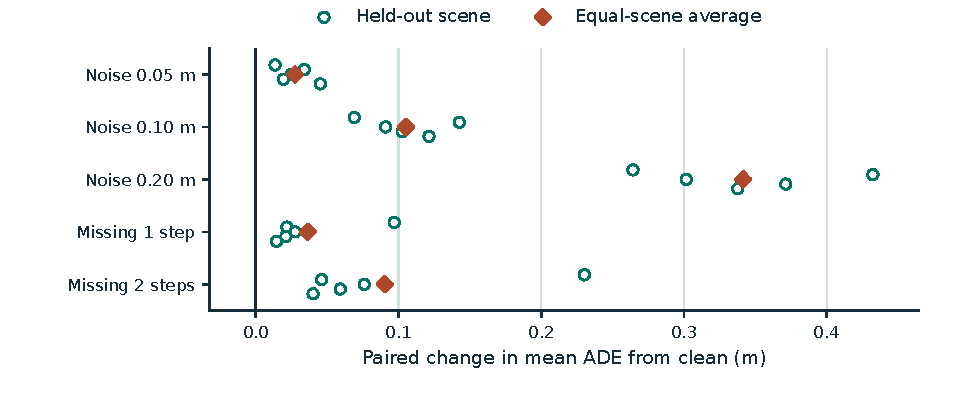
\includegraphics[width=.87\linewidth,height=1.84in,keepaspectratio]{contributions/social_stgcnn/assets/paired_robustness.pdf}
\caption{MeanADE change relative to clean input. Each open circle is a
held-out scene after averaging three seeds. The diamond is the five-scene
average. Only the target's observed history receives the perturbation.}
\label{fig:social_stgcnn_robustness}
\end{figure}

\textbf{Where forecasts miss.}
The two fixed seed-zero examples in Figure~\ref{fig:social_stgcnn_paths}
show different kinds of overshoot. The ETH pedestrian slows and changes
direction. The Univ pedestrian ends 0.89\,m from the last observed point.
Most sampled paths carry the earlier motion forward.
We also selected the window with the highest clean minADE at seed zero.
This Univ pedestrian reversed direction with 23 visible neighbors. The
closest endpoint among all twenty draws still missed by 9.52\,m.

\begin{figure}[H]
\centering
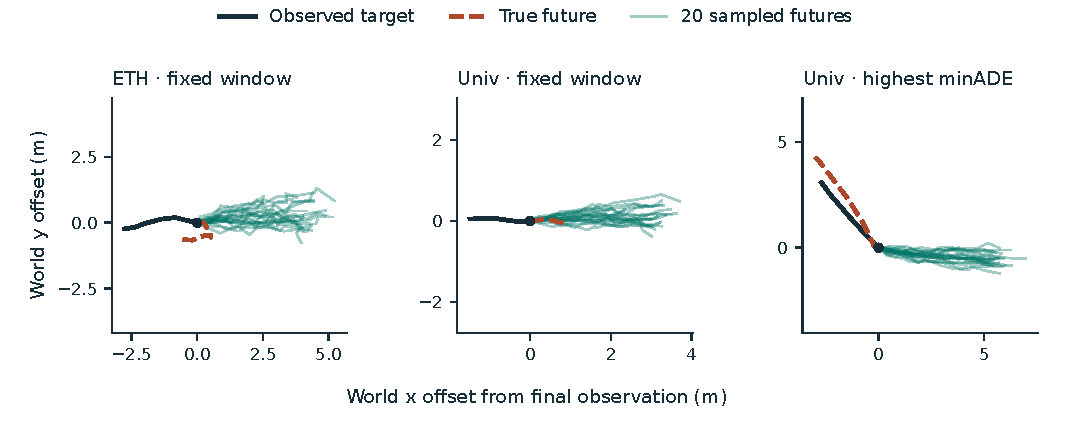
\includegraphics[width=.96\linewidth,height=2.12in,keepaspectratio]{contributions/social_stgcnn/assets/trajectories.pdf}
\caption{The first two windows were fixed before formal scoring. The last
panel was selected by error. Coordinates are centered on the last observed
position, with equal horizontal and vertical units within each panel.
The panels have separate axis ranges.}
\label{fig:social_stgcnn_paths}
\end{figure}

\textbf{Crowd size, motion and cost.}
Clean meanADE was 0.702\,m for the 119 windows without a visible neighbor
and 1.005\,m for the 29,105 windows with at least eight. The former group
covers four scenes, while the latter includes all 24,334 Univ windows.
Crowd size and scene composition vary together. On clean inputs, the
within-window 99th percentile of sampled acceleration exceeded its
training-derived threshold in 95.8\% of windows after equal-fold aggregation.
For groups of contemporaneous targets, the minimum pair distance over the
twelve steps fell below the fold's training fifth-percentile distance in
a mean fraction of 0.886 of draw indices. These proximity statistics
combine independently sampled targets.

On one two-thread Linux CPU allocation, the median end-to-end latency per
128 fixed targets was \ModelRuntime{social_stgcnn}{end_to_end_ms}\,ms.
Median preprocessing took \ModelRuntime{social_stgcnn}{preprocessing_ms}\,ms,
including discovery of visible neighbors. Graph inference and sampling
took \ModelRuntime{social_stgcnn}{prediction_sampling_ms}\,ms. For
the first 32 eligible targets with at least eight neighbors, end-to-end
time ranged from 6.47\,ms on Zara1 to 86.55\,ms on Univ. The runtime
tables retain the individual folds, populations and measurement boundaries.
